\documentclass{article}
\usepackage{graphicx}
\usepackage{hyperref}
\usepackage{xcolor}

\graphicspath{ {images/} }
\begin{document}
\pagecolor{white}

\title{%
  Comparison of symmetric ciphers in OpenSSL \\
  \large HWI - CNS Sapienza}

\author{Giulio Serra 1904089}
\date{November 4, 2019}

\maketitle

\begin{titlepage}
\end{titlepage}

\tableofcontents

\begin{titlepage}
\end{titlepage}

\section{Introduction}\label{sec:intro}

This essay aims to evaluate the performances of different OpenSSL ciphers using the Java environment and the the Cipher class.\\
\\The evaluation of the performances is based on a rateo between the encryption of two text files(100 kb and 1Mb) and their decryption, computed using a generated key with the maximum length supported by each cipher.\\\\The e/d rateo compute the average time of each cipher varying the operating mode between CBC(Cipher Block Chaining) and ECB(Electronic Codebook).


\section{Ciphers}\label{sec:ciphers}
	
	The list of cipher tested for the purpose of this essay includes:
	
	
	\subsection{AES}
	AES - (short for Advanced Encryption Standard) is a symmetrical key block cipher developed by 		Vincent Rijmen and Joan Daemen chosen by NIST to became the new encryption standard 		overtaking DES published in the 70s.\\
	\\It operates using key of 128 bit to a maximum of 256 bit in length bringing the total possible 		attempts for a brute force attack to vary from $2^{128}$ to $2^{256}$.
	The decryption of the algorithm is based on the substitution and permutation network, meaning that 
	the encryption takes the plain text and the key and using a series of linked mathematical operations to output a cipher text.\\
	 In the case of AES those mathematical operations consist in:\\
	 \\- SubBytes: where each byte in the state array is replaced with a byte from a lookup table.\\
 \\- ShiftRow: each bytes in each row of the state are shifted cyclically to the left. \\
	 \\- AddRoundKey: each byte of the state is combined with a byte of the round subkey using the XOR operation.\\
	 
	\subsection{DES}
	DES (short for Data Encryption Standard) is is a symmetrical key block encryption algorithm developed in the early 1970s at IBM and based on an earlier design by Horst Feistel. \\It's based on a 56 bit key + 8 parity bits , the 	unusual key length comes from the fact that, when designed, the unreliability of the communication channel played a big role in the development of the algorithm.\\
	\\Because of the small key length (at least compared to other modern algorithm) DES is considered 	insecure (at least when used by itself no more than one time).\\
	\\DES operates by 16 identical stage of processing (where the key is splitted in two chunks of 32 bit each and processed alternately), with two permutation: one at the beginning and one at the end.
	\subsection{Blowfish}
	Blowfish is a symmetrical key block cipher designed in 1993 to replace the aging DES, it uses 32 up to 448 bit keys .\\The encryption uses a 16 round Feistel cipher, (the same as the one used in DES), the cipher need a minimum of 4kb to run, so it can't be used on small embedded systems.
	
	\subsection{RC2}
	RC2 (Short for Rivest Cipher) is a symmetric key block cipher designed by Ron Rivest from 1987, it's  a 64-bit block cipher with a variable size key. \\Its 18 rounds are arranged as a source-heavy unbalanced Feistel network, with 16 rounds of one type (MIXING) punctuated by two rounds of another type (MASHING).
	
	\section{Operating Modes}\label{sec:opMode}
	Operating modes describes how a single block(that usually does not correspond to a single bit but rather multiple bits) in processed in a block cipher.\\ The operation modes gives us a lot informations about confidentiality  and authenticity of the encrypted message.\\ The main parameters to evaluate a cipher block mode are: parallelization of the encryption/decryption process (to make it faster using pipelines) and Random read access. 
	
	\subsection{ECB}
	ECB is short Electronic CodeBook where the message is divided into blocks and each one is encrypted, the disadvantages of this operating modes is the lack of pattern hiding.\\ Because of each chunk is encrypted separately, ECB is very easy to parallelize both in encryption and decryption.
	
	\subsection{CBC}
	CBC is short for Cipher Block Chaining , each block of plaintext is XOR with previous block of encrypted plaintext, so each block depends on the previous one ,because of this design , the encryption cannot be parallelized.\\
 To make every message unique, the chain must be initialized by an Initialization Vector (Seed).  	
	
	\subsection{Padding}
	Because every block cipher works on a fixed size and every message comes in a variety of ways: both ECB and CBC requires that every message needs to be padded to uniform the length of the plain text to be divided in equal blocks.
	
	
\section{Encryption in JAVA}\label{sec:encJava}

The Java Cipher Class(JCC) rappresent the core of the JCE(Java Cryptography Extension), released starting with JAVA 6.
JCC contains utilities to use all the above ciphers varying mode of operations and padding.
The framework provide also methods to generate secure keys suitable for different algorithms.

	\subsection{JCC Initialization}
		The JCC initialization takes a String the rappresent the desired cipher + operating mode in the format of:\\ algorithm/mode/padding, when using CBC you can even specify the Initialization vector (IV) by using the command: \\ 
		
		\begin{verbatim}
			Cipher cipher = Cipher.getInstance(...);
			byte[] iv = new byte[cipher.getBlockSize()]; // initialization vector
				IvParameterSpec ivParams = new IvParameterSpec(iv);
				cipher.init(...);
		\end{verbatim}

	\subsection{Generating a Safe Key}
		JCC provide methods and classes for generating a safe and random key suitable for a selected algorithm: this is done using the KeyGenerator class, for example:
		
		\begin{verbatim}
			KeyGenerator keyGen;
		try {
			keyGen = KeyGenerator.getInstance("algorithm_name");
			keyGen.init("k_length");
			super.safeKey = keyGen.generateKey();
		} catch (NoSuchAlgorithmException e) {
			e.printStackTrace();
		}		\end{verbatim}
		
		the keyGen class is initialized with the algorithm name (for example "AES") and a key length: this parameter also dipend on the selected algorithm(for example AES takes keys 128b to 256b in length).
		
		\subsection{Encrypting and Decrypting}
		
		The encryption takes the plaintext and a key (generated by user or by the framework) and output the cipher text, everything is done by using the cipher.doFinal(plaintext) method:
		
		\begin{verbatim}
			byte[] raw = key.getByteArray();
			
			Key skeySpec = new SecretKeySpec(raw, "algorthm_name");			
			
			Cipher cipher = Cipher.getInstance(getMode());

			if(super.opm == OperatingMode.CBC) {

				byte[] iv = new byte[cipher.getBlockSize()]; // initialization vector
				IvParameterSpec ivParams = new IvParameterSpec(iv);
				cipher.init(Cipher.ENCRYPT_MODE, skeySpec,ivParams);

			}else {
				cipher.init(Cipher.ENCRYPT_MODE, skeySpec);
			}

			byte[] encriptedArray  = cipher.doFinal(plainText);
			
		\end{verbatim}
		
		The decryption works in the opposite way: taking the cipher text and the key, outputting an array of bytes rappresenting the plain text:
		
			\begin{verbatim}
			byte[] raw = key.getByteArray();
			Key skeySpec = new SecretKeySpec(raw, "algorthm_name);
			
			
			Cipher cipher = Cipher.getInstance(getMode());

			if(super.opm == OperatingMode.CBC) {

				byte[] iv = new byte[cipher.getBlockSize()];
				IvParameterSpec ivParams = new IvParameterSpec(iv);
				cipher.init(Cipher.DECRYPT_MODE, skeySpec,ivParams);

			}else {
				cipher.init(Cipher.DECRYPT_MODE, skeySpec);
			}

			byte[] decriptedArray  = cipher.doFinal(cipherText);
			
		\end{verbatim}
		
		\section{Designing a Common Interface}\label{sec:designcInterface}
		
		When developing a OOP we need to design code suitable for both user and developers in the sense that someone that want to use our library/program doesn't want to know all the technical details of every piece of code, but rather just use it to perform operations, we also want to maximize the recycle of the code to prevent spreading of errors.\\ So it's a wise choice to design a common interface across all the algorithms to expose to the user just the needed informations: every algorithms just encrypt/decrypt a stream of bytes using a key, so we need to implement a class with all the basic informations common among all the ciphers, then each one will extends that class implementing the cipher's algorithm:
		
		\begin{figure}[h]
		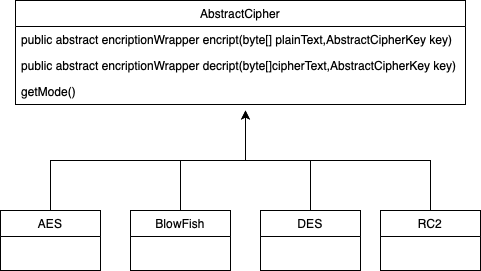
\includegraphics[width=0.5\textwidth ]{images/AbstractCipher.png}
		\centering
		\caption{Class Diagram for AbstractCipher}
	\end{figure}

in the same way we need to define a common class for a key used by the ciphers: while every algorithm use a key to encrypt/decrypt, the format may vary, so every ciphers implements a method to validate it:

		
		\begin{figure}[h]
		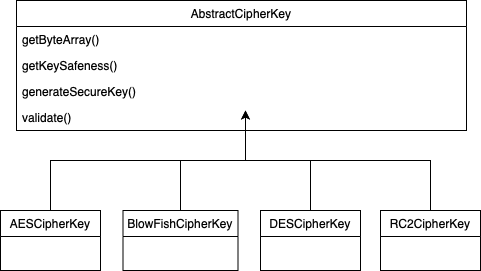
\includegraphics[width=0.5\textwidth ]{images/AbstractKey.png}
		\centering
		\caption{Class Diagram for AbstractCipherKey}
		\end{figure}

	
In addition, we need to define two more classes: one to parse the two text files(PlainText.java), and the other to take the elapsed time(StopWatch.java).


	\section{The Performance Test}\label{sec:encJava}
		Running the main.java file instantiate 4 different ciphers running both in ECB and CBC, each encryption and decryption return a wrapper containing the e/d data and the elapsed time.Here is a piece of the output of an execution:
		
		\begin{verbatim}
------------------------------------------------------------
Starting AES encryption (unsafe key) in CBC mode. (AES/CBC/PKCS5Padding)
Encryption ended. Elapsed Time: 0.085s
encrypted message length: 96144
------------------------------------------------------------
------------------------------------------------------------
Starting AES decryption in CBC mode. (AES/CBC/PKCS5Padding)
Elapsed Time: 0.007s
decrypted message length: 96140
------------------------------------------------------------
Now decrypting AES with a safe key:
------------------------------------------------------------
Starting AES encryption (safe key) in CBC mode. (AES/CBC/PKCS5Padding)
Encryption ended. Elapsed Time: 0.001s
encrypted message length: 96144
------------------------------------------------------------
------------------------------------------------------------
Starting AES decryption in CBC mode. (AES/CBC/PKCS5Padding)
Elapsed Time: 0.002s
decrypted message length: 96140
------------------------------------------------------------
------------------------------------------------------------
Starting AES encryption (unsafe key) in ECB mode. (AES/ECB/PKCS5Padding)
Encryption ended. Elapsed Time: 0.001s
encrypted message length: 96144
------------------------------------------------------------
------------------------------------------------------------
Starting AES decryption in ECB mode. (AES/ECB/PKCS5Padding)
Elapsed Time: 0.002s
decrypted message length: 96140
------------------------------------------------------------
Now decrypting AES with a safe key:
------------------------------------------------------------
Starting AES encryption (safe key) in ECB mode. (AES/ECB/PKCS5Padding)
Encryption ended. Elapsed Time: 0.001s
encrypted message length: 96144
------------------------------------------------------------
------------------------------------------------------------
Starting AES decryption in ECB mode. (AES/ECB/PKCS5Padding)
Elapsed Time: 0.001s
decrypted message length: 96140
------------------------------------------------------------
------------------------------------------------------------
Average AES rateo 0.6666666666666666
------------------------------------------------------------
------------------------------------------------------------
Starting DES encryption (unsafe key) in CBC mode. (DES/CBC/PKCS5Padding)
Encryption ended. Elapsed Time: 0.011s
encrypted message length: 96144
------------------------------------------------------------
------------------------------------------------------------
Starting DES decryption in CBC mode. (DES/CBC/PKCS5Padding)
Elapsed Time: 0.006s
decrypted message length: 96140
------------------------------------------------------------
....Other ciphers and modes...
	\end{verbatim}

An execution print the elapsed time of e/d in seconds, the length of e/d message and the average rateo of the cipher computed considering all the operating modes of the cipher(ECB and CBC):
	
	\begin{verbatim}
	 *Give the average speed of encription 
	 */
	public static double getAverageSpeedRateo() {

		try {
			AES aes_cbc = new AES(OperatingMode.CBC);
			aes_cbc.print = false;

			AES aes_ecb = new AES(OperatingMode.ECB);
			aes_ecb.print = false;

			AESCipherKey key = new AESCipherKey("");
			key.generateSecureKey();


			AbstractCipher.encriptionWrapper cbc_encripted= aes_cbc.encript(PlainText.getInstance().getBytesArray(),key);
			AbstractCipher.encriptionWrapper cbc_decripted = aes_cbc.decript(cbc_encripted.data,key);

			AbstractCipher.encriptionWrapper ecb_encripted= aes_ecb.encript(PlainText.getInstance().getBytesArray(),key);
			AbstractCipher.encriptionWrapper ecb_decripted = aes_ecb.decript(ecb_encripted.data,key);

			double avg_encription = (cbc_encripted.elapsedSeconds + ecb_encripted.elapsedSeconds)/2;
			double avg_decription = (cbc_decripted.elapsedSeconds + ecb_decripted.elapsedSeconds)/2;

			return avg_encription/avg_decription;



		} catch (Exception e) {
			return 0.0;
		}

	}
	\end{verbatim}

	Taking a closer look to the execution: the program deem as unsafe every key created by the user, that's because as stated in section 4.2, the JCC can auto generate safe keys for every cipher.
\\An user provided key is not safe because it could be guessed with a brute force attack, with less attempts, taking informations from dictionaries containing common used words.\\\\\\\\\\

	\section{Test Results}\label{sec:trTest}
	
	Here are the plots of 5 different executions of the four algorithms:
	
	\begin{figure}[h]
		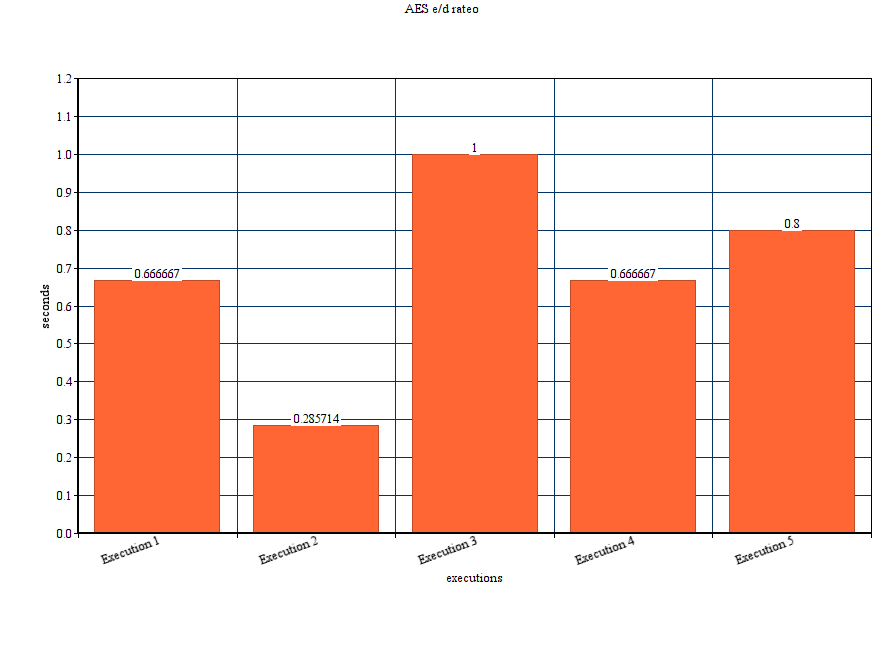
\includegraphics[width=1\textwidth ]{images/AES_ed.png}
		\centering
		\caption{AES (small file) executions}
	\end{figure}
	
	\begin{figure}[h]
		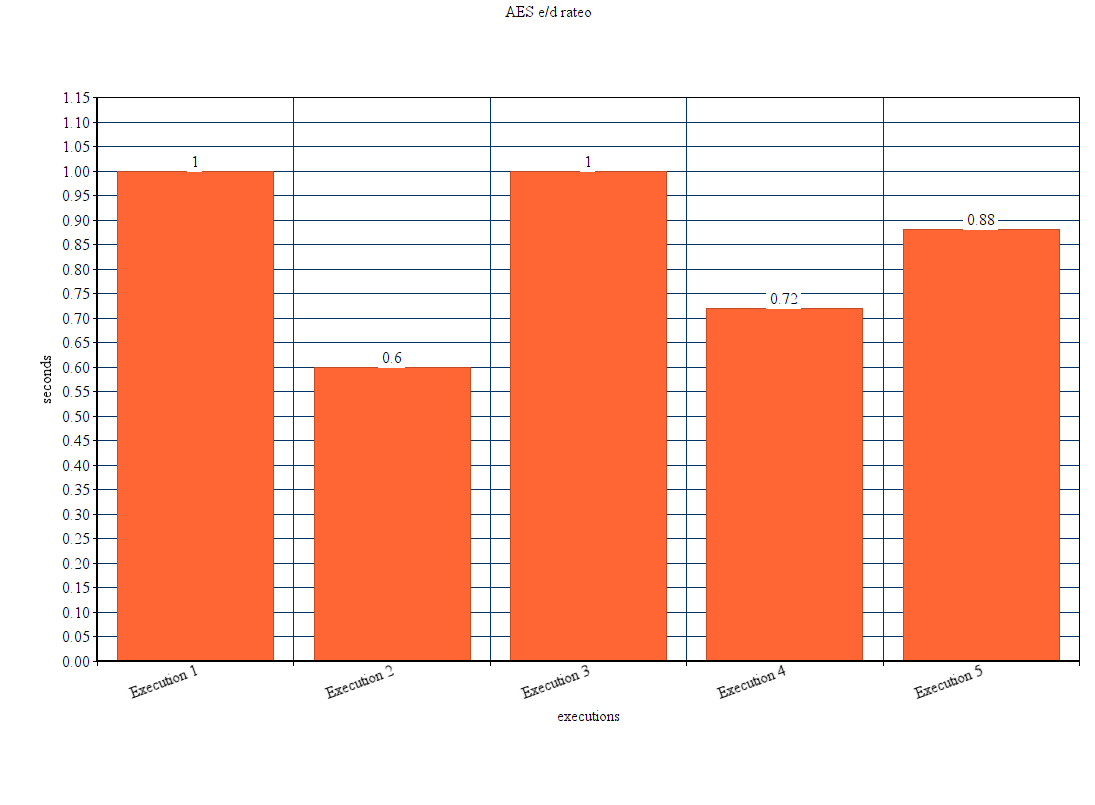
\includegraphics[width=1\textwidth ]{images/AES(big).png}
		\centering
		\caption{AES (big file) executions}
	\end{figure}
	
	\begin{figure}[h]
		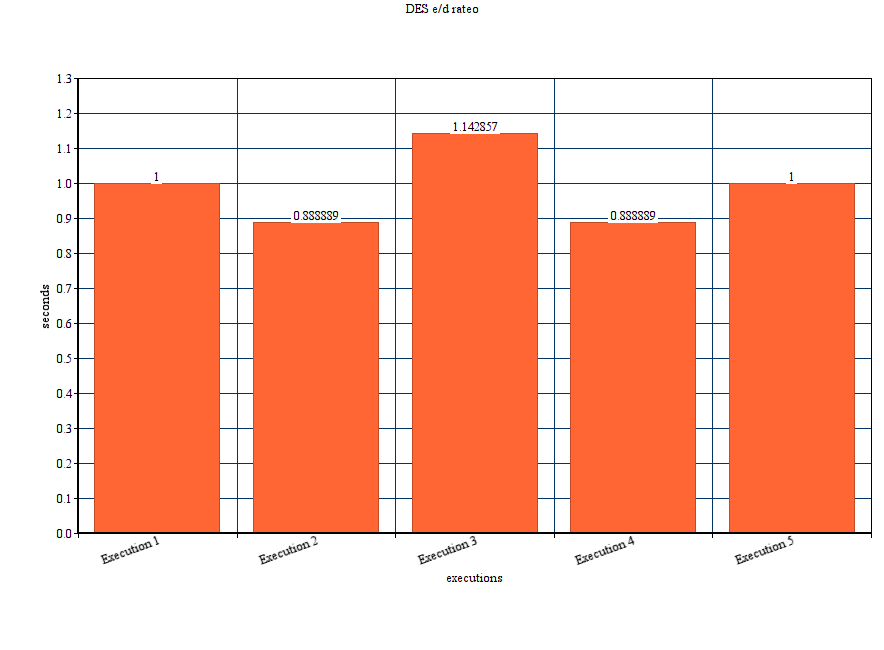
\includegraphics[width=1\textwidth ]{images/DES_ed.png}
		\centering
		\caption{DES (small file) executions}
	\end{figure}
	
	\begin{figure}[h]
		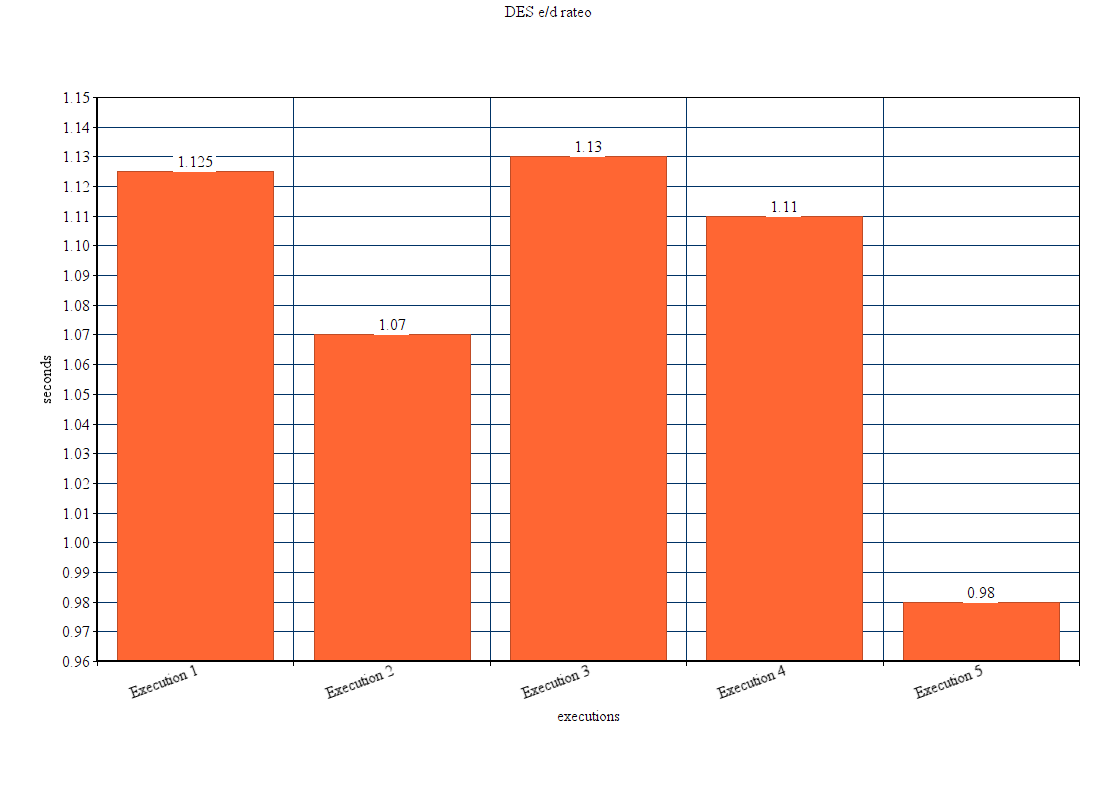
\includegraphics[width=1\textwidth ]{images/DES(big).png}
		\centering
		\caption{DES (big file) executions}
	\end{figure}
	
	\begin{figure}[h]
		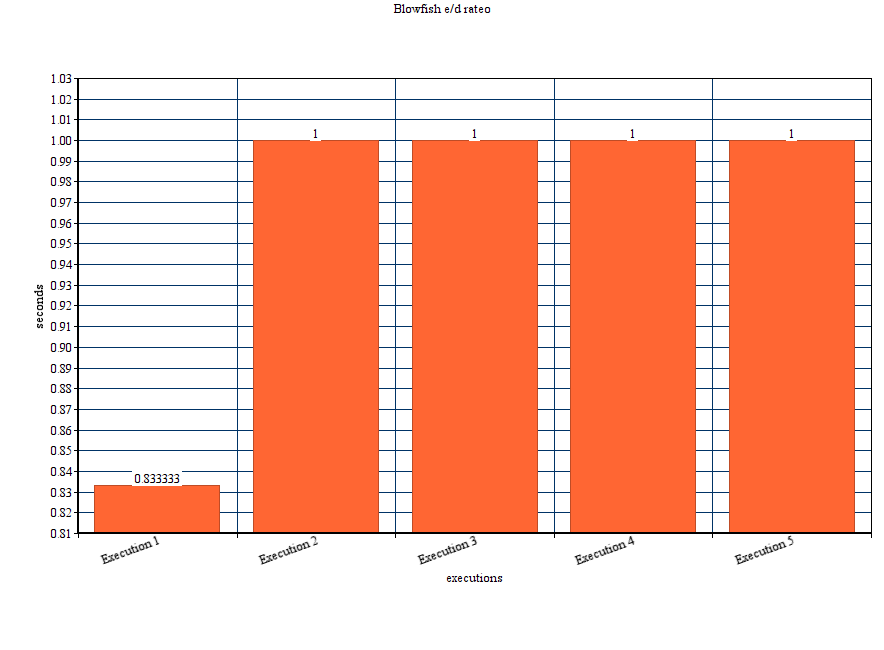
\includegraphics[width=1\textwidth ]{images/Blowfish.png}
		\centering
		\caption{Blowfish (small file) executions}
	\end{figure}
	
	\begin{figure}[h]
		\includegraphics[width=1\textwidth ]{images/Blowfish(big).png}
		\centering
		\caption{Blowfish (big file) executions}
	\end{figure}

	\begin{figure}[h] 
		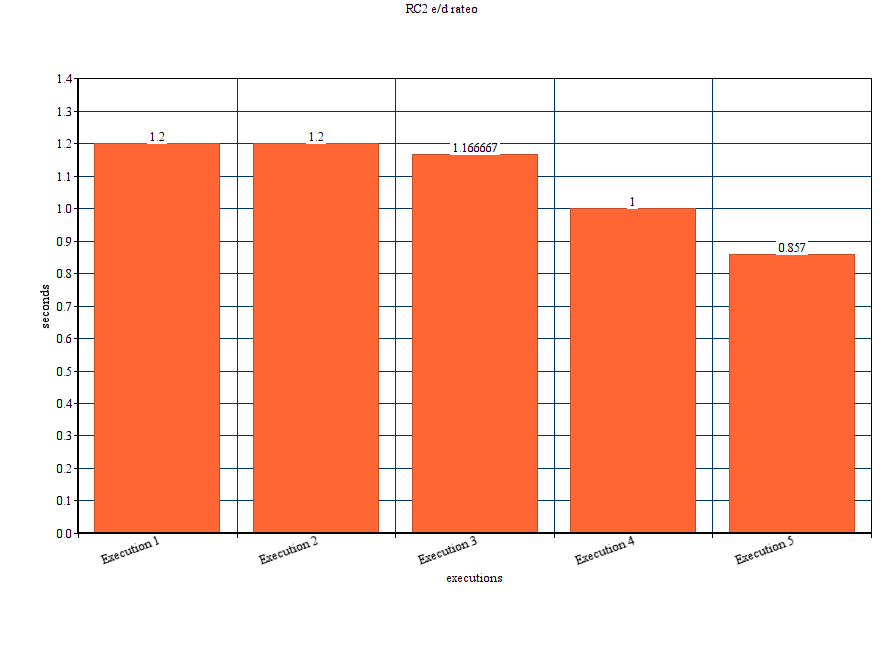
\includegraphics[width=1\textwidth ]{images/RC2.png}
		\centering
		\caption{RC2 (small file) executions}
	\end{figure}
	
	\begin{figure}[h] 
		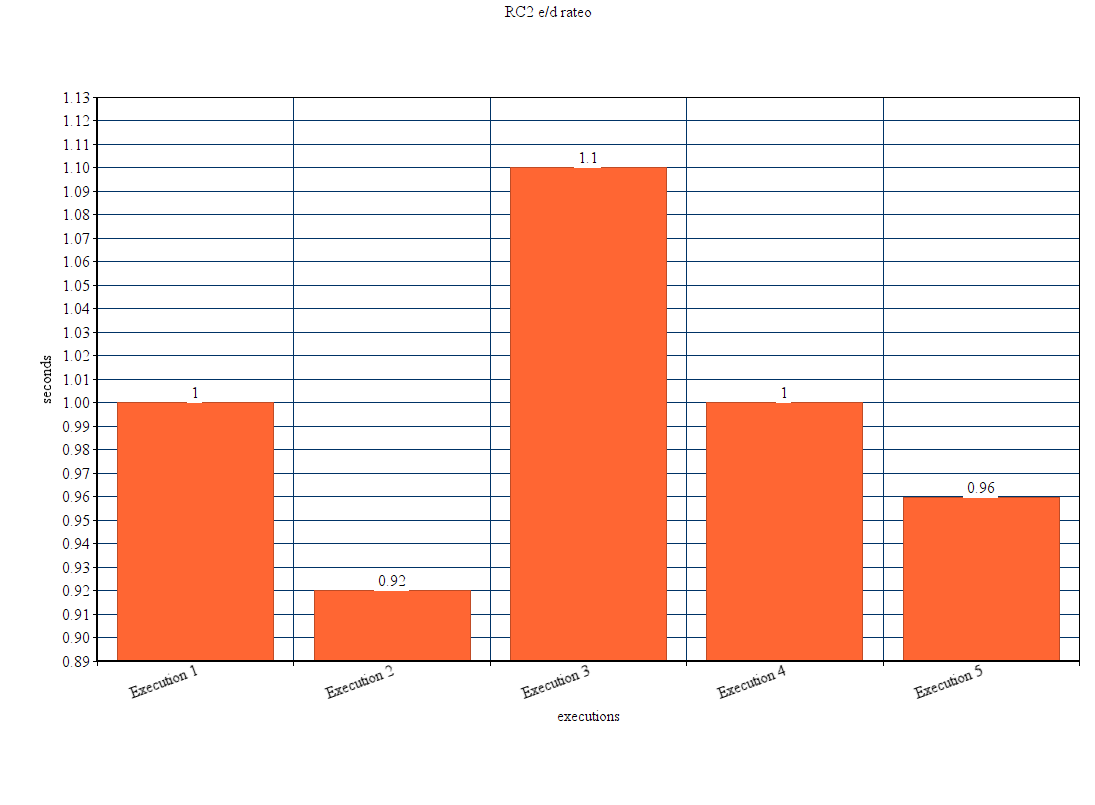
\includegraphics[width=1\textwidth ]{images/RC2(big).png}
		\centering
		\caption{RC2 (big file) executions}
	\end{figure}
	
	\clearpage
	
	AES keeps its rateo below 1 across all the five execution, with an average encryption speed of
	0.1s in CBC mode and 0.003s in ECB(it can be parallelized), while it took  0.01s for decryption in 	CBC and 0.003s in ECB mode.\\
	
	DES struggle to keep the rateo below 1 (spiking to 1.14s): with an average of encryption time of 
	0.04 for CBC and 0.01 in ECB while decryption is around 0.02 for CBC and 0.014s in ECB.
	The decryption time are quite poor even compared to AES , that even operates on a minimum of 	128b long keys (long as twice as a DES key).\\

	Blowfish keeps more or less consistent through all the 5 executions, keeping the rateo in exactly 1 	while the encryption time is 0.008s in CBC and 0.01 in ECB. For decryption 0.011 in CBC and 
	0.008s in ECB.\\
	
	RC2's rateo decrease whit every executions, while the encryption time remain consistent with 		CBC and ECB, the same for decryption: 0.02s for both CBC and ECB.\\

	\section{Final Considerations}\label{sec:trFinalConsid}
	While both Blowfish and RC2 output some good performance, their small key size rappresent 		a major problem in terms of brute force attacks and birthdays attacks: Blowfish in particular with a 	minimum needed memory of 4kb is not suitable for use on small devices(such as embedded systems). AES, on the other hand, is quite resistant to attacks (with it's 128b key size) and small e/d rateo, quite fast(so is good for network needs) and not particularly resource consuming(so very good for mobile devices).\\ DES has poor performances: with and e/d rateo of 1 or more(while having a key of just 64 bytes) and is even notorious for not being resistant to brute force attacks.

	\section{References}\label{sec:ref}
	
	Java Cipher class: \url{https://docs.oracle.com/javase/7/docs/api/javax/crypto/Cipher.html}
	
	
	
		
\end{document}